% Document commands
% --- Auxiliary functions ---

% --- Settinge ---
\newcommand{\bracketed}[1]{\left[#1\right]}

% --- General ---
% Absolute value
\NewDocumentCommand{\abs}{m}{
    % #1: argument
    \left\vert#1\right\vert
}

% --- Linear Algebra ---
% Inner product
\NewDocumentCommand{\iprod}{o m m}{
    % #1: the domain (for integration)
    % #2: argument 1
    % #3: argument 2
    \left(#2,\: #3\right)\IfValueT{#1}{_{#1}}
}

\NewDocumentCommand{\iprodS}{o m m}{
    % #1: the domain (for integration)
    % #2: argument 1
    % #3: argument 2
    \left\langle#2,\: #3\right\rangle\IfValueT{#1}{_{#1}}
}

% Norm
\NewDocumentCommand{\norm}{o m}{
    % #1: Specifier of the norm
    % #2: argument
    \left\vert\left\vert#2\right\vert\right\vert\IfValueT{#1}{_{#1}}
}

% --- Basic tensor functions
% Transposition
\NewDocumentCommand{\transpT}{o m}{
    % #1: Indices of the transposition
    % #2: The tensor
    #2\IfNoValueTF{#1}{^\mathrm{T}}{^{\overset{#1}{\mathrm{T}}}}
}

% % The trace
% \NewDocumentCommand{\tr}{o m}{
%     % #1: True, if brackets should be used
%     % #2: The tensor
%     \mathrm{tr}\IfNoValueTF{#1}{\: #2}{\bracketed{#2}}
% }

% Additive decomposition
\NewDocumentCommand{\sym}{o m}{
    % #1: True, if brackets should be used
    % #2: The tensor
    \mathrm{sym}\IfNoValueTF{#1}{\: #2}{\bracketed{#2}}
}

\NewDocumentCommand{\skw}{o m}{
    % #1: True, if brackets should be used
    % #2: The tensor
    \mathrm{skw}\IfNoValueTF{#1}{\: #2}{\bracketed{#2}}
}

% \NewDocumentCommand{\as}{o m}{
%     % #1: True, if brackets should be used
%     % #2: The tensor
%     \mathrm{as}\IfNoValueTF{#1}{\: #2}{\bracketed{#2}}
% }

% Determinant
\NewDocumentCommand{\determ}{o m}{
    % #1: True, if brackets should be used
    % #2: The tensor
    \mathrm{det}\IfNoValueTF{#1}{\: #2}{\bracketed{#2}}
}

% Inverse
\NewDocumentCommand{\inv}{o m}{
    % #1: True, if brackets should be used
    % #2: The tensor
    \IfNoValueTF{#1}{#2 ^{-1}}{\bracketed{#2}^{-1}}
}

\NewDocumentCommand{\invt}{o m}{
    % #1: True, if brackets should be used
    % #2: The tensor
    \IfNoValueTF{#1}{#2 ^{-\mathrm{T}}}{\bracketed{#2}^{-\mathrm{T}}}
}

% --- Analysis ---
% Gradient and Divergence 
\newcommand{\grad}{\nabla\:}
\renewcommand{\div}{\nabla\cdot}

\NewDocumentCommand{\divc}{o m m}{
    % #1: True, if brackets should be used
    % #2: The arguemnt
    % #3: Configuration, within which the divergence is evaluated
    \nabla_{\vec{#3}} \cdot \IfNoValueTF{#1}{#2}{\bracketed{#2}}
}

\NewDocumentCommand{\gradc}{o m m}{
    % #1: True, if brackets should be used
    % #2: The arguemnt
    % #3: Configuration, within which the divergence is evaluated
    \nabla_{\vec{#3}} \: \IfNoValueTF{#1}{#2}{\bracketed{#2}}
}

% Integrational domains
\newcommand{\dInt}[1]{\;\mathrm{d}#1}
\newcommand{\dVol}{\;\mathrm{d}v}
\newcommand{\dVolR}{\;\mathrm{d}V}
\newcommand{\dSurf}{\;\mathrm{d}a}
\newcommand{\dSurfR}{\;\mathrm{d}A}

% Material timederivative
\NewDocumentCommand{\mtDiff}{o m}{
    % #1: True, if brackets should be used
    % #2: The arguemnt
    \IfNoValueTF{#1}{#2'}{\left(#2\right)'}
}

% Gateaux derivative
\newcommand{\dGat}[2]{\mathrm{D}_{#2}\left[#1\right]}

% Linearisation
\newcommand{\Lin}[1]{\mathrm{LIN}\left[#1\right]}

% --- Function spaces ---
\NewDocumentCommand{\VecSpace}{o o o m}{
    % #1: The domain
    % #2: The boundary condition
    % #3: The dimension
    % #4: The function-space
    \IfNoValueTF{#3}
    {\mathrm{#4} \IfValueT{#2}{_{#2}} \ifthenelse{\equal{#1}{}}{}{\left(#1\right)}}
    {\left( \mathrm{#4} \IfValueT{#2}{_{#2}} \ifthenelse{\equal{#1}{}}{}{\left(#1\right)} \right) ^{#3}}
}

\NewDocumentCommand{\LiiSpace}{o o o}{
    % #1: The domain
    % #2: The boundary condition
    % #3: The dimension
    \IfNoValueTF{#3}
    {\mathrm{L}^2 \IfValueT{#2}{_{#2}} \ifthenelse{\equal{#1}{}}{}{\left(#1\right)}}
    {\left( \mathrm{L}^2 \IfValueT{#2}{_{#2}} \ifthenelse{\equal{#1}{}}{}{\left(#1\right)} \right) ^{#3}}
}

\NewDocumentCommand{\HiSpace}{o o o}{
    % #1: The domain
    % #2: The boundary condition
    % #3: The dimension
    \IfNoValueTF{#3}
    {\mathrm{H}^1 \IfValueT{#2}{_{#2}} \IfValueT{#1}{\left(#1\right)}}
    {\left( \mathrm{H}^1 \IfValueT{#2}{_{#2}}\IfValueT{#1}{\left(#1\right)} \right) ^{#3}}
}

\NewDocumentCommand{\HdivSpace}{o o o}{
    % #1: The domain
    % #2: The boundary condition
    % #3: The dimension
    \IfNoValueTF{#3}
    {\mathrm{H} \IfValueT{#2}{_{#2}} \left(\mathrm{div}\ifthenelse{\equal{#1}{}}{}{,\, #1}\right)}
    {\left( \mathrm{H} \IfValueT{#2}{_{#2}} \left(\mathrm{div}\ifthenelse{\equal{#1}{}}{}{,\, #1}\right) \right) ^{#3}}
}

% --- Finite element spaces ---
\NewDocumentCommand{\sdisc}{m}{
    % #1: The field variable
    #1_{\h}
}

\NewDocumentCommand{\stdisc}{m}{
    % #1: The field variable
    #1_{\h\tau}
}

\NewDocumentCommand{\feP}{o o}{
    % #1: The degree
    % #2: The dimension
    \IfNoValueTF{#2}
    {\mathrm{P} \IfValueT{#1}{_{#1}}}
    {\left( \mathrm{P} \IfValueT{#1}{_{#1}} \right)^{#2}}
}

\NewDocumentCommand{\feDP}{o o}{
    % #1: The degree
    % #2: The dimension
    \IfNoValueTF{#2}
    {\mathrm{DP} \IfValueT{#1}{_{#1}}}
    {\left( \mathrm{DP} \IfValueT{#1}{_{#1}} \right)^{#2}}
}

\NewDocumentCommand{\feRT}{o o}{
    % #1: The degree
    % #2: The dimension
    \IfNoValueTF{#2}
    {\mathrm{RT} \IfValueT{#1}{_{#1}}}
    {\left( \mathrm{RT} \IfValueT{#1}{_{#1}} \right)^{#2}}
}

\NewDocumentCommand{\feBDM}{o o}{
    % #1: The degree
    % #2: The dimension
    \IfNoValueTF{#2}
    {\mathrm{BDM} \IfValueT{#1}{_{#1}}}
    {\left( \mathrm{BDM} \IfValueT{#1}{_{#1}} \right)^{#2}}
}
% --- Matrices and vector definitions ---
\renewcommand{\vec}[1]{\bm{\mathrm{#1}}}
\newcommand{\vecGreek}[1]{\bm{#1}}
\newcommand{\mat}[1]{\bm{\mathrm{#1}}}
\newcommand{\matGreek}[1]{\bm{#1}}

% --- The defined symbols ---
\newcommand{\sbReference}{0}
\newcommand{\sbReferenceSolid}{0\solid}
\newcommand{\spPhase}{\phase}
\newcommand{\spPhaseReal}{\phase\mathrm{R}}
\newcommand{\sbPhase}{\phase}
\newcommand{\spDimension}{d}
\newcommand{\sbElemental}{e}
\newcommand{\spFluid}{\fluid}
\newcommand{\spFluidReal}{\fluid\mathrm{R}}
\newcommand{\sbFluid}{\fluid}
\newcommand{\spDiscrete}{h}
\newcommand{\spEqlb}{\mathrm{R}}
\newcommand{\spSolid}{\solid}
\newcommand{\spSolidExtra}{\solid\mathrm{E}}
\newcommand{\spSolidReal}{\solid\mathrm{R}}
\newcommand{\sbSolid}{\solid}
\newcommand{\gdim}{d}
\newcommand{\elmt}{e}
\newcommand{\h}{h}
\newcommand{\eqlb}{\mathrm{R}}
\newcommand{\defCauchyGreenRight}{\mat{C}}
\newcommand{\strainGreenLagrange}{\mat{E}}
\newcommand{\YoungsMod}{\mathrm{E}}
\newcommand{\DefGrad}{\mat{F}}
\newcommand{\stressPKi}{\mat{P}}
\newcommand{\stressPKii}{\mat{S}}
\newcommand{\xRef}{\vec{X}}
\newcommand{\xCur}{\vec{x}}
\newcommand{\CsbS}{\mat{C}_{\solid}}
\newcommand{\EsbS}{\mat{E}_{\solid}}
\newcommand{\YoungsModspS}{\mathrm{E}^{\solid}}
\newcommand{\FsbS}{\mat{F}_{\solid}}
\newcommand{\PispS}{\mat{P}^{\solid}}
\newcommand{\PispSE}{\mat{P}^{\solid\mathrm{E}}}
\newcommand{\PispF}{\mat{P}^{\fluid}}
\newcommand{\PiispS}{\mat{S}^{\solid}}
\newcommand{\PiispSE}{\mat{S}^{\solid\mathrm{E}}}
\newcommand{\PiispF}{\mat{S}^{\fluid}}
\newcommand{\XsbPhase}{\vec{X}_{\phase}}
\newcommand{\XsbS}{\vec{X}_{\solid}}
\newcommand{\XsbF}{\vec{X}_{\fluid}}
\newcommand{\xsbPhase}{\vec{x}_{\phase}}
\newcommand{\xsbS}{\vec{x}_{\solid}}
\newcommand{\xsbF}{\vec{x}_{\fluid}}
\newcommand{\strainGreenLagrangeLin}{\matGreek{\varepsilon}}
\newcommand{\Lamei}{\lambda}
\newcommand{\Lameii}{\mu}
\newcommand{\PoissonsRatio}{\nu}
\newcommand{\stressPKLin}{\matGreek{\sigma}}
\newcommand{\LinEsbS}{\matGreek{\varepsilon}_{\solid}}
\newcommand{\lispS}{\lambda^{\solid}}
\newcommand{\liispS}{\mu^{\solid}}
\newcommand{\nuspS}{\nu^{\solid}}
\newcommand{\LinPKspS}{\matGreek{\sigma}^{\solid}}
\newcommand{\LinPKspSE}{\matGreek{\sigma}^{\solid\mathrm{E}}}
\newcommand{\LinPKspF}{\matGreek{\sigma}^{\fluid}}
\newcommand{\LinPKEqlb}{\matGreek{\sigma}^{\mathrm{R}}}
\newcommand{\LinPKEqlbH}{\matGreek{\sigma}^{\mathrm{R}}_\h}
\newcommand{\Displacement}{\vec{u}}


\newcommand{\domain}{\Omega}
\newcommand{\domainH}{\mathcal{T}_{\h}}

\newcommand{\patch}{\omega_{z}}
\newcommand{\hatfunc}{\varphi_{z}}

\newcommand{\GenSol}{\mathrm{u}}
\newcommand{\GenSolH}{\mathrm{u}_\h}

\newcommand{\flux}{\vecGreek{\varsigma}}
\newcommand{\fluxH}{\vecGreek{\varsigma}\left(\GenSolH\right)}
\newcommand{\fluxHi}{\vecGreek{\varsigma}\left(\GenSolH\right)\big\vert_i}

\newcommand{\fluxR}{\vecGreek{\varsigma}^\spEqlb}
\newcommand{\fluxRH}{\vecGreek{\varsigma}^\spEqlb_\h}
\newcommand{\fluxRHz}{\vecGreek{\varsigma}^\spEqlb_{\h,z}}
\newcommand{\fluxRHzSEi}{\Delta\widetilde{\bm{\varsigma}}^R_{z,h}}
\newcommand{\fluxRHzSEii}{\Delta\bm{\varsigma}^R_{z,h}}
\newcommand{\fluxRHi}{\vecGreek{\varsigma}^\spEqlb_\h\big\vert_i}
\newcommand{\fluxRHziSEi}{\Delta\widetilde{\bm{\varsigma}}^R_{z,h}\big\vert_i}
\newcommand{\fluxRHziSEii}{\Delta\bm{\varsigma}^R_{z,h}\big\vert_i}

\newcommand{\LinPKEqlbHz}{\matGreek{\sigma}^{\mathrm{R}}_{z,\h}}
\newcommand{\LinPKEqlbHzSEi}{\Delta\widetilde{\matGreek{\sigma}}^{\mathrm{R}}_{z,\h}}
\newcommand{\LinPKEqlbHzSEii}{\Delta\matGreek{\sigma}^{\mathrm{R}}_{z,\h}}
\newcommand{\LinPKEqlbHzWS}{\Delta_\mathrm{sym}\matGreek{\sigma}^{\mathrm{R}}_{z,\h}}

% Write the full path to the location of the graphics relative to book.tex
\graphicspath{{chapters/brodbeck/graphics/}}

\title{Adaptive finite element methods based on flux equilibration using FEniCSx}
\titlerunning{Adaptive finite element methods based on flux equilibration using FEniCSx}

\author{Maximilian Brodbeck, Fleurianne Bertrand and Tim Ricken}
\authorrunning{Brodbeck et al.}

\institute{Maximilian Brodbeck, Tim Ricken \email{{brodbeck, ricken}@isd.uni-stuttgart.de} \at Institute of Structural Mechanics and Dynamics, University of Stuttgart\\
Fleurianne Bertrand \email{fleurianne.bertrand@mathematik.tu-chemnitz.de} \at Faculty of Mathematics, University of Technology Chemnitz}

\maketitle

\abstract{A-poteriori error estimates and resulting adaptive finite element schemes allow for the determination of solutions with predefined accuracy, while preserving optimal convergence orders. An important class of guaranteed, robust error upper bounds, mostly in the energy norm, are based on so called equilibarted fluxes. This contribution shows how such fluxes -- H(div) functions fulfilling the problems underlying conservation law -- can be calculated in FEniCSx. Therefore, dolfinx\_eqlb is introduced, its algorithmic structure is described and classical benchmarks for adaptive solution procedures for the Poisson problem and linear elasticity are presented.}

\section*{Introduction}
The accurate resolution of physical quantities in numerical simulations is of significant importance across various fields of engineering and applied sciences. 
Therefore, various software packages have been proposed, while the latest trend -- followed e.g. by FEniCSx (see \cite{FEniCSx_2023}) -- focuses on abstraction, generality and automation without losing computational efficiency. 
It is well known that on general domains, numerical solutions often lack the regularity, required to directly apply a priori estimates. 
To maintain optimal convergence, adaptive procedures based on a posteriori error estimates, combined with local mesh refinement, have been developed. 
FEniCS is currently well-suited for handling residual-based error estimators, error estimates based on the strategy by Bank and Weiser proposed by \cite{Bulle_BankWeiserApeFenics_2021} or automated, goal oriented strategies introduced by \cite{Rognes_AutomatedEE_2013}, making it a valuable tool for many adaptive finite element methods. 
However, posteriori error estimates involves the equilibration of flux or stress, leading to guaranteed, fully localised, and easily computable error upper bounds, especially in the energy norm, are still missing.
Rooted in the hypercircle identity of \cite{Prager_Equilibartion_1947}, the Poisson problem is discussed in works such as \cite{Braess_EqlbFluxes_2008}, \cite{Cai_SemiexplzEqlb_2012}, \cite{Ern_FluxEqlb_2015} or \cite{Bertrand_Hypercircle_2020} while applications to linear elasticity can be found e.g. in \cite{Bertrand_EqlbElast_2021}.
Addressing this gap, dolfinx\_eqlb, a library for the computation of equilibrated fluxes and stresses, is introduced.
Following the philosophy of the FEniCS project, performance-relevant routines are written in c++ and can be used in Python via their appropriate bindings. 
This contribution starts with a review of error estimates and requirements on the equilibration process. 
The basic algorithmic structure of dolfinx\_eqlb is then discussed, and two benchmarks for adaptive finite element methods demonstrate the capabilities of the library.
\vspace{-0.5cm}

\section*{A-posteriori error estimation based on equilibrated fluxes}
\textbf{Equilibration in presence of the full gradient} starts from the Poisson problem
\begin{equation}
    \div\flux(\GenSol) = \mathrm{f} \;\text{in}\; \domain \quad\text{with}\quad \flux(\GenSol) := -\kappa\,\grad \GenSol \quad\text{and}\quad 
    \begin{cases}
        \GenSol = 0                    & \text{on} \; \Gamma_\mathrm{D}\\
        \flux(\GenSol)\cdot\vec{n} = 0 & \text{on} \; \Gamma_\mathrm{N}\\
    \end{cases}\; .
    \label{eq:poisson}
\end{equation}
For any $\mathrm{f} \in \LiiSpace[\domain]$, the weak solution $\GenSol \in \HiSpace[\domain][\Gamma_\mathrm{D}]$ -- the Sobolev space of functions in $\HiSpace[\domain]$ with prescribed values on the Dirichlet boundary $\Gamma_\mathrm{D}$ -- satisfies
\begin{equation}
    \iprod{\flux(\GenSol)}{\grad\mathrm{v}} = \iprod{\mathrm{f}}{\mathrm{v}} \quad\text{for all}\quad \mathrm{v} \in \HiSpace[\domain][\Gamma_\mathrm{D}]\; .
    \label{eq:poisson_weak}
\end{equation}
Following \cite{Braess_EqlbFluxes_2008} or \cite{Ern_FluxEqlb_2015}, an improved flux, fulfilling the so called Prager-Synge identity is introduced.
\begin{definition}
    An equilibrated flux $\fluxR\in \Sigma(\Omega)$, with $\VecSpace[\domain]{\Sigma} := \{\vec{v} \in \HdivSpace[\domain]:\, \vec{v}\cdot\vec{n} = 0 \;\text{on}\; \Gamma_\mathrm{N} \}$ being the space of functions in H(div) with zero-trace on the Neumann boundary $\Gamma_\mathrm{N}$, fulfils
    \begin{equation}
        \iprod{\div\fluxR}{\mathrm{q}} = \iprod{\mathrm{f}}{\mathrm{q}} \quad\text{for all}\quad \mathrm{q} \in \div \Sigma(\Omega) \;\text{in }\; \Omega\ .
        \label{eq:flux_eqlb_conditions} 
    \end{equation}
    \label{def:equilibrated_flux}
\end{definition}
\vspace{-0.6cm}

Defining the space $\VecSpace[]{V}_k := \left\{\mathrm{v}_\h \in \HiSpace[\domain]:\, \mathrm{v}_\h\vert_\mathrm{T} \in \feP[k](\mathrm{T})
\right\}$ with $\feP[k](\mathrm{T})$ being the cell-wise polynomials of degree $k$, $\GenSol$ can be approximated in $\VecSpace[]{V}_{\Gamma ,k}  := \VecSpace[]{V}_{k} \cap \HiSpace[\domain][\Gamma_\mathrm{D}]$.
For any arbitrary $\GenSolH \in \VecSpace[]{V}_{\Gamma ,k}$ and any equilibrated flux $\fluxR \in \VecSpace[\domain]{\Sigma}$ the Prager-Synge identity
\begin{equation}
    \iprod{\delta\flux}{\grad\delta\GenSol} = \iprodS[\partial\domain]{\delta\flux\cdot\vec{n}}{\delta\GenSol} - \iprod{\div\delta\flux}{\delta\GenSol} = 0\; ,
    \label{eq:prager_synge_identity}
\end{equation}
with $\delta\flux = \flux(\GenSol) - \fluxR$ respectively $\delta\GenSol = \GenSol - \GenSolH$ is satisfied.
Defining further $\feRT[m]$, the Raviart-Thomas space of order $m$, an upper bound on the error in a scaled $\mathrm{H}^1$ norm holds.
\begin{theorem}
    Let $\kappa$ be piecewise constant, $\GenSol \in \HiSpace[\domain][\Gamma_\mathrm{D}]$ be the solution of \eqref{eq:poisson_weak}, $\GenSolH \in \VecSpace[]{V}_{\Gamma ,k}$ be arbitrary and $\fluxRH\in\feRT[m]$ be an equilibrated flux, then
    \begin{equation}
        \norm{\kappa^{1/2}\grad\bracketed{\GenSol - \GenSolH}}^2 \leq \sum_{\mathrm{T}\in\domainH} \bracketed{\norm[\mathrm{T}]{\kappa^{-1/2}\bracketed{\fluxRH - \fluxH}} + C_P \norm[\mathrm{T}]{\mathrm{f} - \div\fluxRH}}^2\; .
        \label{eq:ee_poisson-disc-kappa}
    \end{equation}
    \label{thm:ee_poisson}
\end{theorem}

\vspace{-0.7cm}
A proof can be found in \cite{Cai_SemiexplzEqlb_2012}.

\textbf{Equilibration in presence of the symmetric gradient} $\strainGreenLagrangeLin(\Displacement) = \sym{\grad\Displacement}$ considers the linearised Piola-Kirchhoff stress $\stressPKLin(\Displacement) = 2\strainGreenLagrangeLin(\Displacement) + \tilde{\Lamei}\,\div\Displacement\,\mat{I}$ which enters the balance of linear momentum
\begin{equation}
    \div\stressPKLin(\Displacement) = -\vec{f} \;\text{in}\; \domain \quad\text{with}\quad \Displacement = \vec{0} \; \text{on} \; \Gamma_\mathrm{D}  \quad\text{and}\quad \stressPKLin(\Displacement) \cdot \vec{n} = \vec{t} \; \text{on} \; \Gamma_\mathrm{N}\; .
    \label{eq:linear_elasticity}
\end{equation}
\noindent For any $\vec{f} \in \LiiSpace[\domain]$, the weak solution $\Displacement \in \HiSpace[\domain][\Gamma_\mathrm{D}][2]$ fulfills
\vspace{-0.25cm}
\begin{equation}
    \iprod{\stressPKLin(\Displacement)}{\strainGreenLagrangeLin(\vec{v})} = \iprod{\vec{f}}{\vec{v}} - 
    \iprodS[\Gamma_\mathrm{N}]{\vec{t}}{\vec{v}}
    \quad\text{for all}\quad \vec{v} \in \HiSpace[\domain][\Gamma_\mathrm{D}][2]\; .
    \label{eq:linear_elasticity-weak}
\end{equation}
Considering the symmetry of the stress tensor in a weak sense as in \cite{Bertrand_EqlbElast_2021}, the following definition of the equilibrated stress tensor is introduced. 
Therein $\Pi_{m-1}\left(\bullet\right)$ denotes the projection of a function into a cell-wise polynomial space of order $m-1$.
\begin{definition}
An equilibrated stress is a function $\LinPKEqlbH\in\feRT[m][2]$ 
    fulfilling
    \begin{equation}
        \div\LinPKEqlbH = -\Pi_{m-1}\,\vec{f}\;\text{on}\;\domain \quad\text{respectively}\quad \LinPKEqlbH \cdot \vec{n} = \vec{t} \; \text{on} \; \Gamma_\mathrm{N}\; ,
        \label{eq:stress_eqlb_conditions}
    \end{equation}
    and the weak symmetry condition $ \iprod{\sigma^\spEqlb_\h\big\vert_{12} - \sigma^\spEqlb_\h\big\vert_{21}}{\gamma_\h} = 0 \quad\text{for all}\quad \gamma_\h \in \VecSpace[]{V}_{1}$.
    \label{def:equilibrated_stress}
\end{definition}
While the error is measured in the energy norm $\vert\vert\vert \bullet \vert\vert\vert^2 = \norm{\strainGreenLagrangeLin\left(\bullet\right)}^2 + \tilde{\Lamei}\,\norm{\div\left(\bullet\right)}^2$, the operator $\displaystyle \mathcal{A}\left(\bullet\right) = \frac{1}{2}\bracketed{\left(\bullet\right) - \frac{\tilde{\Lamei}}{2\,(1+\tilde{\Lamei})}\tr{\left(\bullet\right)}\,\mat{I}}$ with norm $\norm[\mathcal{A}]{\left(\bullet\right)}^2 = \iprod{\left(\bullet\right)}{\mathcal{A}\left(\bullet\right)}$ allows for a robust error control.
\vspace{-0.25cm}
\begin{theorem}
    Let $\Displacement \in \HiSpace[\domain][\Gamma_\mathrm{D}][2]$ be the solution of \eqref{eq:linear_elasticity-weak}, $\Displacement_\h \in \left(\VecSpace[]{V}_{\Gamma ,k}\right)^2$ be arbitrary, and $\LinPKEqlbH$ be an equilibrated stress. For $\delta\Displacement = \Displacement - \Displacement_\h$ it holds
    \begin{equation}
        \vert\vert\vert \delta\Displacement \vert\vert\vert^2 \leq \norm[\mathcal{A}]{\LinPKEqlbH - \stressPKLin(\Displacement_\h)}^2 + C_K \sum_{\mathrm{T}\in\domainH} \bracketed{\norm[\mathrm{T}]{\skw{\LinPKEqlbH}} + C_P \norm[\mathrm{T}]{\vec{f} + \div\LinPKEqlbH}}^2\; .
        \label{eq:ee_linelasticity}
    \end{equation}
    \label{thm:ee_linear_elasticity}
\end{theorem}
\vspace{-0.6cm}
\begin{proof}
    Evaluating the $\mathcal{A}$-norm of the $\LinPKEqlbH - \stressPKLin(\Displacement_\h)$ yields
    \begin{equation}
        \norm[\mathcal{A}]{\LinPKEqlbH - \stressPKLin(\Displacement_\h)} \geq \vert\vert\vert \delta\Displacement \vert\vert\vert^2 +\norm{\strainGreenLagrangeLin\left(\delta\Displacement\right)}^2 - 2\,\iprod{\delta\stressPKLin^\spEqlb}{\strainGreenLagrangeLin\left(\delta\Displacement\right)}\; ,
        \label{eq:proof_ee-le_eval_anorm}
    \end{equation}
    where $\delta\stressPKLin^\spEqlb$ denotes the difference between true- and equilibrated stress $\stressPKLin(\Displacement) - \LinPKEqlbH$. 
    Integration by parts under consideration of the symmetry of the true stress and the equilibration conditions \eqref{eq:stress_eqlb_conditions} allows a reformulation of the mixed term:
    \begin{equation}
        \iprod{\delta\stressPKLin^\spEqlb}{\strainGreenLagrangeLin\left(\delta\Displacement\right)} = \iprod{\vec{f} + \div\LinPKEqlbH}{\delta\Displacement} + \iprod{\skw{\LinPKEqlbH}}{\grad\delta\Displacement}\; .
        \label{eq:proof_ee-le_reformulation}
    \end{equation}
    Based on the weak symmetry, \eqref{eq:proof_ee-le_reformulation} can be bounded from above
    \begin{equation}
        \iprod{\delta\stressPKLin^\spEqlb}{\strainGreenLagrangeLin\left(\delta\Displacement\right)} \leq C_K \sum_{\mathrm{T}\in\domainH} \bracketed{\norm[\mathrm{T}]{\skw{\LinPKEqlbH}} + C_P \norm[\mathrm{T}]{\vec{f} + \div\LinPKEqlbH}}^2 + \norm{\strainGreenLagrangeLin\left(\delta\Displacement\right)}\; .
        \label{eq:proof_ee-le_bound_one}
    \end{equation}
    Inserting \eqref{eq:proof_ee-le_bound_one} into \eqref{eq:proof_ee-le_eval_anorm} completes the proof.
\end{proof}

\section*{Algorithms and implementation}
This section introduces dolfinx\_eqlb, a FEniCSx based library for flux and stress equilibration. 
In order to keep the presentation general, $\bm{\theta}$ denotes in the following either a flux or a stress. 
Adaptive finite element methods are typically based on the loop\\
\vspace{0.15cm}
\centerline{$...$ $\rightarrow$ SOLVE $\rightarrow$ ESTIMATE $\rightarrow$ MARK $\rightarrow$ REFINE $\rightarrow$ $...$}
\vspace{0.15cm}
Using equilibration based error estimates requires the following during the step ESTIMATE:
\begin{enumerate}
    \item The evaluation of projections of the right-hand-side (RHS) $\Pi_{m-1}\,\mathrm{f}$ and the approximated flux $\Pi_{m-1}\,\bm{\theta}_\h$ in a discontinuous Lagrange space of order $m-1 \geq k-1$.
    \item The calculation of the equilibrated flux $\bm{\theta}^\spEqlb_\h\in\feRT[m][d]$.
\end{enumerate}
Therefore, the constrained minimisation problem
\begin{equation}
    \bm{\theta}^\spEqlb_\h = \arg\underset{\vec{v} \in \feRT[m][d] \land\,\mathrm{CONSTR}}{\min} \norm{\vec{v} - \bm{\theta}_\h}
    \label{eq:eqlb_by_global_minimisation}
\end{equation}
is considered, where the constraints $\mathrm{CONSTR}$ and dimension $d$ follow from Definition \ref{def:equilibrated_flux} or \ref{def:equilibrated_stress}.
As a global solution of \eqref{eq:eqlb_by_global_minimisation} is computationally too expensive, the problem is localised by introducing for each node $z$ the nodal, piece-wise linear basis-function $\hatfunc$. 
The support of $\hatfunc$ is denoted as patch $\patch$ and allows for the definition of the local function space
\begin{equation*}
    \mathrm{V}_m(\patch) := \left\{\vec{v}\in\feRT[m][d]:\; \vec{v}\cdot\vec{n}=
    \begin{cases}
        0                                          &  \partial\patch \cap \Gamma_\mathrm{N} = \emptyset\\
        \hatfunc\,\tilde{\mathrm{t}} & \text{else}\;
    \end{cases} 
    \right\}\, .
\end{equation*}
Therein, the projection of the normal trace $\bm{\theta}\cdot\vec{n}$ into the facet-wise polynomial space of order $m-1$ is denoted by $\tilde{\mathrm{t}}$.
Summing up $\bm{\theta}^\spEqlb_{\h,z} \in \mathrm{V}_m(\patch)$ concludes equilibration:
\begin{equation}
    \bm{\theta}^\spEqlb_\h = \sum_z \bm{\theta}^\spEqlb_{\h,z} \; \text{with} \; \bm{\theta}^\spEqlb_{\h,z} := \arg\underset{\vec{v} \in \mathrm{V}_m(\patch) \land \mathrm{CONSTR}}{\min} \norm[\patch]{\vec{v} - \hatfunc\bm{\theta}_\h}\; .
    \label{eq:eqlb_by_local_minimisation}
\end{equation}

Stresses can be handled similarly as fluxes, where -- in a first step -- each row of a stress tensor is treated as an independent flux. 
The weak symmetry condition is enforced in a second step.
Algorithm \ref{alg:eqlb_mesh_level} describes the therefore required structure on the mesh level.
Starting with lists of DOLFINx functions for the equilibrated fluxes $\left\{\fluxRHi\right\}$, the projected fluxes $\left\{\Pi_{m-1}\,\fluxHi\right\}$, the projected RHS $\left\{\Pi_{m-1}\,\mathrm{f}_i\right\}$ and the facets ($fct$) on the Dirichlet boundary of the primal problem $\left\{fct\in\Gamma_\mathrm{D}\right\}$ a general patch is created, which has to be updated for each mesh node.
It serves as sub-mesh respectively sub-function-space required for flux equilibration and the enforcement of the weak symmetry condition.

The patch-local Algorithms for flux equilibration \ref{alg:eqlb_se_patch_level} and enforcement of the weak symmetry condition \ref{alg:eqlb_ws_patch_level} are discussed in the following.
\begin{algorithm}
    \caption{Equilibration on the mesh level.}
    \label{alg:eqlb_mesh_level}

    % Special commands
    \SetKwInOut{Input}{input }

    % The algorithm
    \Input{$\left\{\fluxRHi\right\}$, $\left\{\Pi_{m-1}\,\fluxHi\right\}$, $\left\{\Pi_{m-1}\,\mathrm{f}_i\right\}$ and $\left\{fct\in\Gamma_\mathrm{D}\right\}$}

    \BlankLine
    $patch$ $\gets$ $\mathrm{Patch}\left(mesh, \left\{fct\in\Gamma_\mathrm{D}\right\}, function\_spaces\right)$\;

    \BlankLine
    \For{$i = 0;\ i < n_\mathrm{nodes};\ i++$}
    {
        $patch$.create\_subdofmap($n$)\;
        equilibrate\_flux\_semiexplt(...) \tcp*{see Algorithm \ref{alg:eqlb_se_patch_level}}
        \textbf{if} \textit{weaksym\_stresses} \textbf{then} impose\_weak\_symmetry(...) \tcp*{see Algorithm \ref{alg:eqlb_ws_patch_level}}
    }
\end{algorithm}

\textbf{Flux equilibration} requires the solution of a series of constrained minimisation problems \eqref{eq:eqlb_by_local_minimisation}.
This can be done directly as in \cite{Ern_FluxEqlb_2015} or by splitting the process into an explicit part, followed by an unconstrained minimisation \cite[Appendix A]{Bertrand_HHO_2023}. 
Restricting this discussion on the second approach, the difference of equilibrated- and approximated flux is calculated in two steps:
\begin{equation}
    \fluxRHi - \hatfunc\fluxHi = \fluxRHziSEi + \fluxRHziSEii\; .
    \label{eq:eqlb_se_split}
\end{equation}
While the determination of $\fluxRHzSEi$ is an interpolation-like task, $\fluxRHzSEii$ is determined on a patch-wise divergence free space
\begin{equation*}
    \mathrm{V}^\Delta_m(\patch) := \left\{\vec{v} \in \feRT[m]:\; \div\vec{v}=0 \land \vec{v}\cdot\vec{n}=0 \;\text{on}\; \partial\patch\setminus\Gamma_\mathrm{D} \right\}\; \,
    \label{eq:patchwise_div_free_RT}
\end{equation*} 
from the unconstrained minimisation problem
\begin{equation}
    \iprod[\patch]{\fluxRHzSEii}{\vec{v}_{z,\h}} = -\iprod[\patch]{\fluxRHzSEi}{\vec{v}_{z,\h}} \quad\text{for all}\quad \vec{v}_{z,\h} \in \mathrm{V}^\Delta_m(\patch) \; .
    \label{eq:eqlb_se_unconstrained_min}
\end{equation}
The required hierarchic definition of the Raviart-Thomas space is implemented using Basix's (\cite{Basix_2022}) custom element.

From an algorithmic perspective, the semi-explicit equilibration is performed on each patch for multiple RHS simultaneously.
Beside of patches attached to the boundary $\Gamma_\mathrm{N}$, this allows to assemble the system matrix $\mat{A}$ and compute its Cholesky decomposition only once per patch and reuse it for the different RHS. 
The solution procedure is detailed in Algorithm \ref{alg:eqlb_se_patch_level}.
\begin{algorithm}
    \caption{Function: equilibrate\_flux\_semiexplt}
    \label{alg:eqlb_se_patch_level}

    % Special commands
    \SetKwInOut{Input}{input }
    \SetKwFunction{cPatch}{Patch}\SetKwFunction{cpatch}{patch}

    % The algorithm
    \Input{$\left\{\fluxRHi\right\}$, $\left\{\Pi_{m-1}\,\fluxHi\right\}$, $\left\{\Pi_{m-1}\,\mathrm{f}_i\right\}$}

    \For{$i = 0;\ i < n_\mathrm{RHS};\ i++$}
    {
        Evaluate $\fluxRHziSEi$: \cite[Algorithm 2]{Bertrand_HHO_2023} using $\Pi_{m-1}\,\fluxHi$ and $\mathrm{f}_i$\;
        \BlankLine
        \uIf{$i = 0$}
        {
            Assemble $\mat{A}$ and $\vec{L}$ simultaneously and factorise $\mat{A}$\;
        }
        \Else
        {
            \lIf{$\partial\patch \cap \Gamma_\mathrm{N} = \emptyset $}
            {
                Re-assemble $\vec{L}$
            }
            \lElse
            {
                Assemble $\mat{A}$ and $\vec{L}$ simultaneously and factorise $\mat{A}$
            } 
        }
        \BlankLine
        Evaluate: $\mat{A}\cdot\fluxRHziSEii = \vec{L}$ and append solution: $\fluxRHi \mathrel{+}= \fluxRHziSEi + \fluxRHziSEii$\;
    }
\end{algorithm} 

\textbf{The weak symmetry condition} is enforced by an additional correction term. 
Equilibrating the rows of the stress tensor independently in a first step, results in a stress tensor, fulfilling divergence- and boundary conditions.
Adding $\LinPKEqlbHzWS$ yields
\begin{equation}
    \LinPKEqlbHz - \hatfunc\LinPKEqlbH = \LinPKEqlbHzSEi + \LinPKEqlbHzSEii + \LinPKEqlbHzWS\; ,
\end{equation} 
fulfilling the weak symmetry condition.
Based on $\mat{J}(\bullet)=\begin{pmatrix} 0 & -1\\ 1 & 0 \end{pmatrix}\cdot (\bullet)$ and
\begin{equation*}
    \mathrm{V}_{1,0}(\patch) := \left\{\mathrm{v}_\h \in \HiSpace[\domain]:\, \mathrm{v}_\h\vert_\mathrm{T} \in \feP[k](\mathrm{T}) \land \iprod[\patch]{\mathrm{v}}{1} = 0 \;\text{if}\; \partial\patch \cap \Gamma_\mathrm{D} = \emptyset
    \right\}\; ,
\end{equation*}
the constrained solution $\left( \LinPKEqlbHzWS,\,\xi_{z,\h}\right) \in \mathrm{V}^\Delta_m(\patch) \times \mathrm{V}_{1,0}(\patch)$ satisfies
\begin{equation}
    \begin{split}
        \iprod[\patch]{\LinPKEqlbHzWS}{\bm{\tau}_{z,\h}} + \iprod[\patch]{\mat{J}\left(\xi_{z,\h}\right)}{\bm{\tau}_{z,\h}} = 0\\
        \iprod[\patch]{\LinPKEqlbHzWS}{\mat{J}\left(\gamma_{z,\h}\right)} = -\iprod[\patch]{\LinPKEqlbHzSEi + \LinPKEqlbHzSEii}{\mat{J}\left(\gamma_{z,\h}\right)}\; ,
    \end{split}
    \label{eq:eqlb_ws_constrmin}
\end{equation}
for all $\left(\tau_{z,\h},\,\gamma_{z,\h}\right) \in \mathrm{V}^\Delta_m(\patch)\times\mathrm{V}_{1,0}(\patch)$.

\cite{Bertrand_EqlbElast_2021} proved the solvability of \eqref{eq:eqlb_ws_constrmin}, if patches have at least two internal facets, and $k,m \geq 2$.
In order to avoid the direct solution of
\begin{equation}
    \begin{bmatrix}
        \mat{A} & \mat{0} & \mat{B}_1 & \mat{0} \\
        \mat{0} & \mat{A} & \mat{B}_2 & \mat{0} \\
        \transpT{\mat{B}_1} & \transpT{\mat{B}_2} & \mat{0} & \vec{C}\\
        \vec{0} & \vec{0} & \transpT{\vec{C}}  & \mat{0}
    \end{bmatrix}\cdot
    \begin{bmatrix}
        \vec{u}_{R1} \\
        \vec{u}_{R2} \\
        \vec{c}\\
        \lambda
    \end{bmatrix}
    =
    \begin{bmatrix}
        \vec{0}\\
        \vec{0}\\
        \vec{L}_c\\
        0
    \end{bmatrix}\; ,
    \label{eq:eqs_ws_constrmin}
\end{equation}
the equation system resulting from the saddle-point problem \eqref{eq:eqlb_ws_constrmin}, a Schur complement based solver is implemented. The vectors $\vec{u}_{R1}$ and $\vec{u}_{R2}$  denote the DOFs for the rows of the stress tensor.
Reusing the Cholesky decomposition of $\mat{A}$, the Schur complement $\mat{S} = \mat{B}_1\,\mat{A}^{-1}\,\transpT{\mat{B}_1} + \mat{B}_2\,\mat{A}^{-1}\,\transpT{\mat{B}_2}$ is calculated. 
Solving $\mat{S}\cdot\vec{c}=\vec{L}_c$ based on its LU decomposition followed by solving $\mat{A}\cdot\vec{u}_{Ri}=-\mat{B}_i\cdot\vec{c}$ gives a notable speed-up compared to a direct solution of \eqref{eq:eqs_ws_constrmin}. 
This procedure is outlined in Algorithm \ref{alg:eqlb_ws_patch_level}.
\begin{algorithm}
    \caption{Function: impose\_weak\_symmetry}
    \label{alg:eqlb_ws_patch_level}
    % Special commands
    \SetKwInOut{Input}{input }
    \SetKwFunction{cPatch}{Patch}\SetKwFunction{cpatch}{patch}

    % The algorithm
    \Input{$\left\{\fluxRHi\right\}$}

    \BlankLine
    \lIf{$\left(\partial\patch \cap \Gamma_\mathrm{N} \neq \emptyset\right)$}
    {
        Assemble $\mat{A}$, $\mat{B}_i$, $\mat{C}$ and $\vec{L}_c$ simultaneously
    }
    \lElse
    {
        Assemble $\mat{B}_i$, $\mat{C}$ and $\vec{L}_c$ simultaneously
    } 

    \BlankLine
    \For{$i = 0;\ i < 2;\ i++$}
    {
        \lIf{$\left(\partial\patch \cap \Gamma_\mathrm{N} \neq \emptyset\right)$}
        {
            Apply BCs and re-factorise $\mat{A}$
        }
        $\mat{S} \mathrel{+}= \transpT{\mat{B}_i}\inv{\mat{A}}\mat{B}_i$\;
    }
    \BlankLine
    Solve: $\mat{S}\cdot\vec{c} = \vec{L}_c$\;
    \BlankLine
    \For{$i = 0;\ i < 2;\ i++$}
    {
        \lIf{$\left(\partial\patch \cap \Gamma_\mathrm{N} \neq \emptyset\right)$}
        {
            Apply BCs and re-factorise $\mat{A}$
        }
        Evaluate: $\mat{A}\cdot\vec{u}_{Ri} = -\mat{B}_i\cdot\vec{c}$\;
    }
    \BlankLine
    Append solution: $\LinPKEqlbHz \mathrel{+}= \LinPKEqlbHzWS$\;
\end{algorithm}
\vspace*{-0.8cm}

\section*{Results}
To illustrate the capabilities of dolfinx\_eqlb, adaptive solution procedures are presented for two characteristic problems.
Primal problems are solved using Lagrangian finite elements of degree $k$.
The performance of an error estimate $\eta$ is characterised based on the efficiency index $ \mathrm{i_{eff}} = \eta/\mathrm{err}$, where $\mathrm{err}$ denotes the true error.

\textbf{Example 1:} The Poisson equation (1.2) is solved on a rectangular domain with different coefficients $\kappa$ in each of the four quadrants.
Two sets of parameters $\kappa_2=\kappa_4=1$ and $\kappa_1=\kappa_3$ with either $\kappa_1=5$ (20 refinement levels) or $\kappa_1=100$ (40 refinement levels) are considered.
Dirichlet BCs according to the analytical solution of \cite{Riviere_ApostPoissonCoeffDG_2003} are prescribed on $\Gamma_\mathrm{D}=\partial\Omega$.
Meshes are refined based on a Dörfler marking strategy with $\theta=0.5$. 

Convergence orders (e.o.c) and efficiency indices after the final refinement step are reported in Fig. \ref{fig:poisson-riviere_results}, while the final meshes for first- and second-order approximations of the case $\kappa_1=100$ are shown in Fig. \ref{fig:poisson-riviere_refmesh-p1} and \ref{fig:poisson-riviere_refmesh-p2}. 
The solutions are in good agreement with results from literature. 
Meshes are refined around the singularity in the centre of the domain and the convergence rates are $\approx-0.5$ for $\GenSolH\in\feP[1]$ and $\approx-1$ for $\GenSolH\in\feP[2]$.
For $\kappa_1 = 100$  a convergence rate $<-1$ indicates a pre-asymptotic state of convergence.
The efficiency of the error estimate \eqref{eq:ee_poisson-disc-kappa} depends on the degree $m$ of the equilibrated flux.
Choosing $m=k+1$ yields efficiency indices close to one for $\kappa_1=5$ and between 1.2 and 1.4 for $\kappa_1=100$. 
For $m=k$ they are slightly worse.
\begin{figure}
    \centering
    \begin{subfigure}[b]{0.32\textwidth}
        \centering
        \begin{tabular}{@{}c|c c|c|c@{}}
            \toprule
            \multicolumn{1}{l}{$\kappa_1$} & $k$ & $m$ & $\mathrm{e.o.c}$ & $\mathrm{i_{eff}}$ \\ \midrule
            \multirow{4}{*}{$5$}     & 1 & 1 & $0.50$ & $1.47$ \\
                                     & 1 & 2 & $0.50$ & $1.06$ \\
                                     & 2 & 2 & $0.99$ & $1.40$ \\
                                     & 2 & 3 & $1.03$ & $1.05$ \\ \cmidrule(l){1-5} 
            \multirow{4}{*}{$100$}   & 1 & 1 & $0.50$ & $1.70$ \\
                                     & 1 & 2 & $0.54$ & $1.26$ \\
                                     & 2 & 2 & $1.36$ & $1.78$ \\
                                     & 2 & 3 & $2.14$ & $1.36$ \\ \cmidrule(l){1-5} 
        \end{tabular}
        \caption{}
        \label{fig:poisson-riviere_results}
    \end{subfigure}
    \hfill
    \begin{subfigure}[b]{0.32\textwidth}
        \centering
        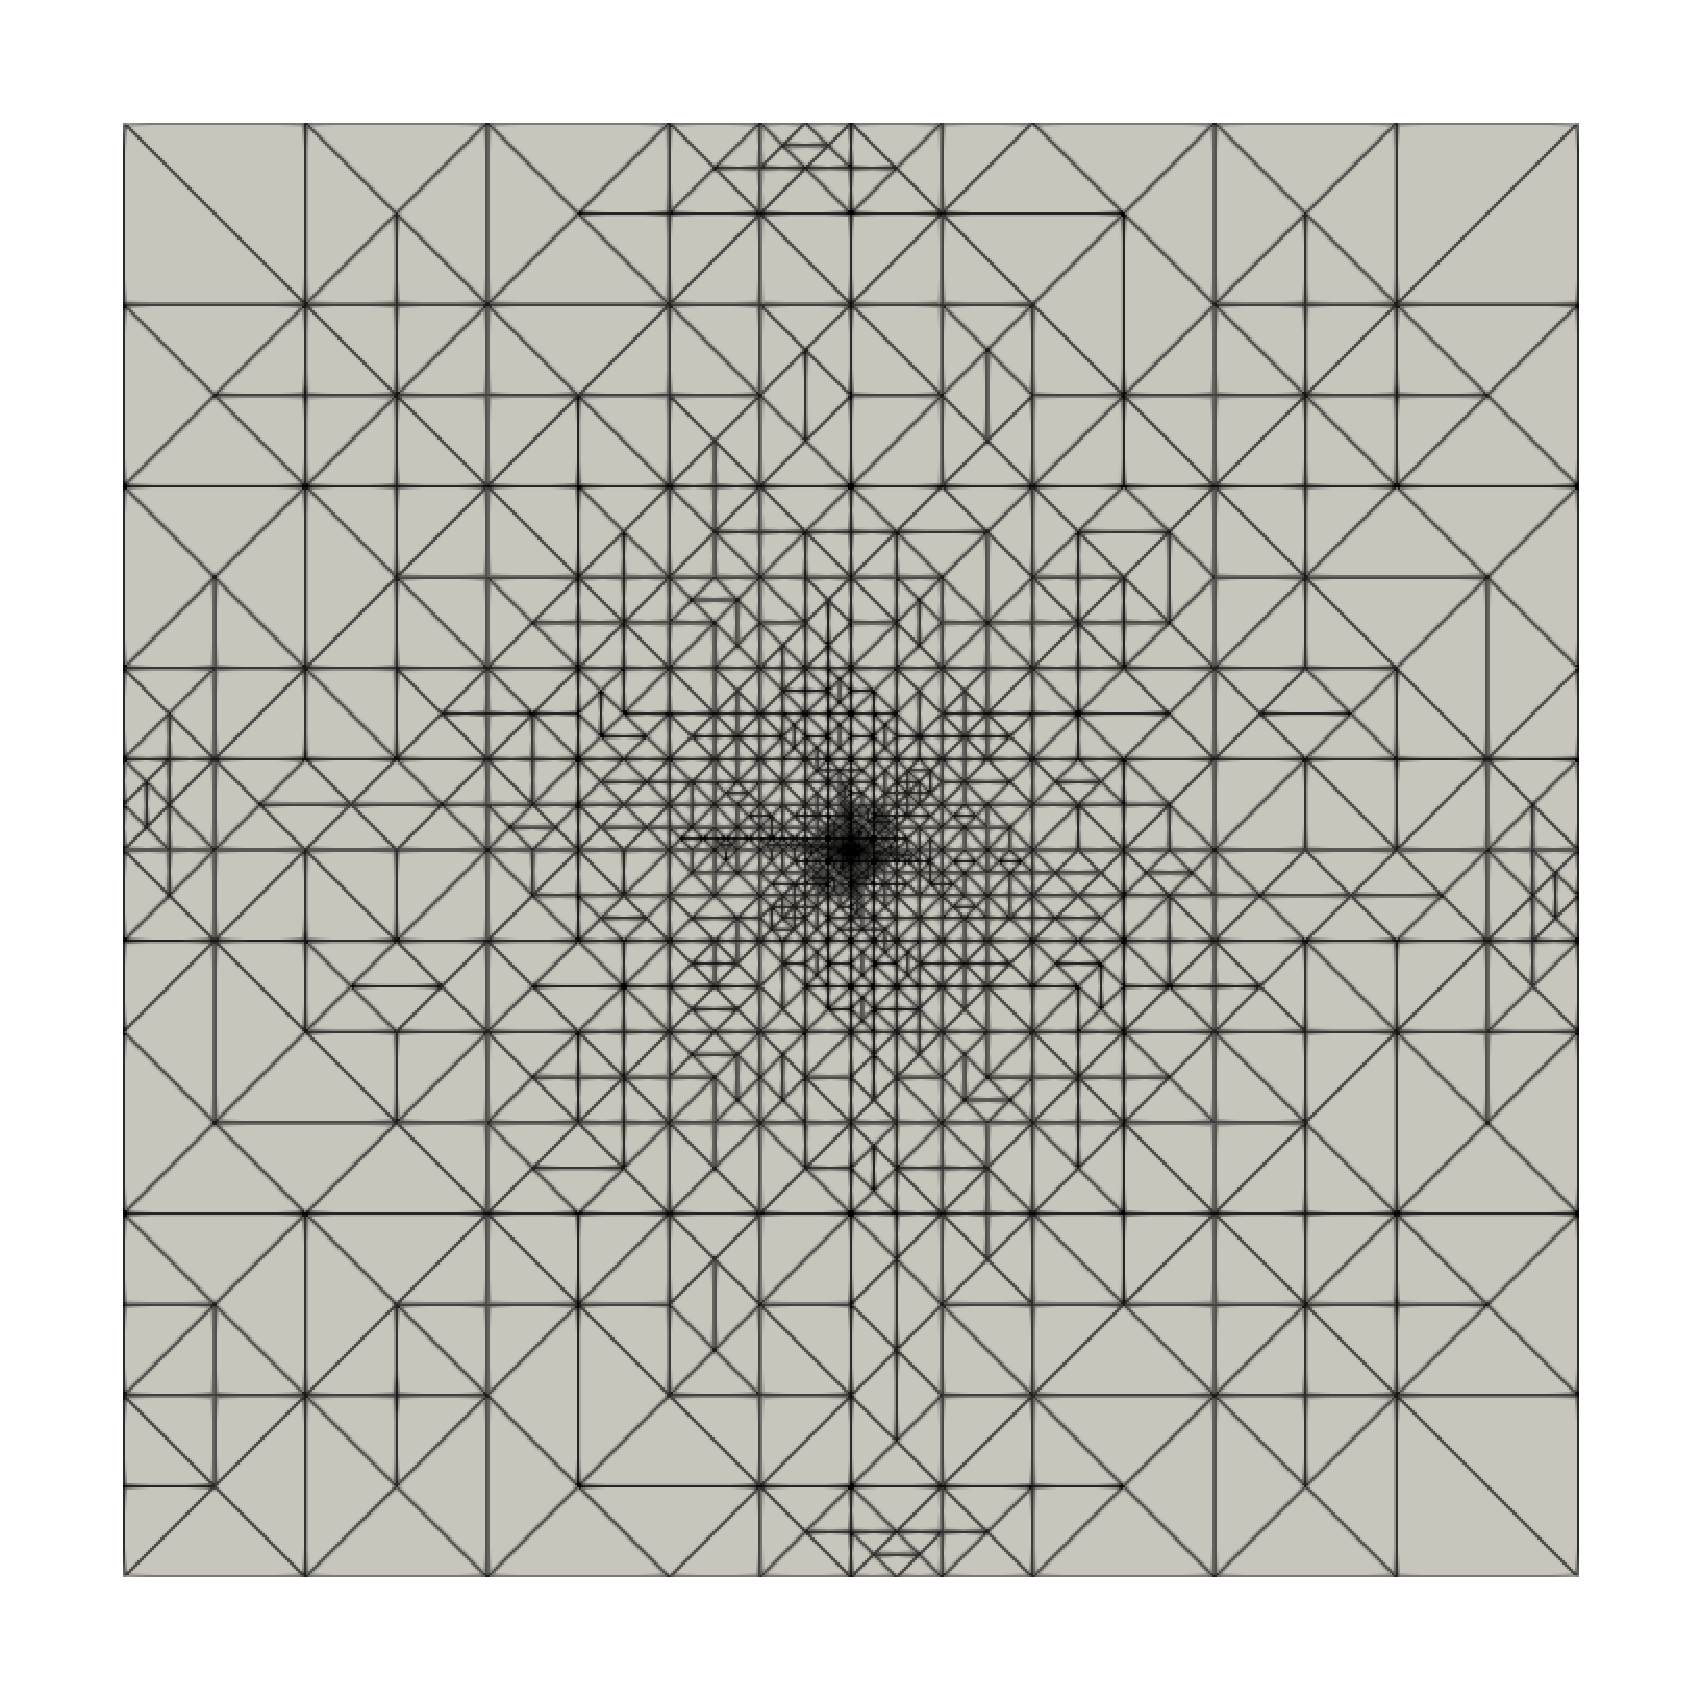
\includegraphics[width=\textwidth]{Riviere-100_P1_RT2_Mesh.pdf}
        \caption{}
        \label{fig:poisson-riviere_refmesh-p1}
    \end{subfigure}
    \hfill
    \begin{subfigure}[b]{0.32\textwidth}
        \centering
        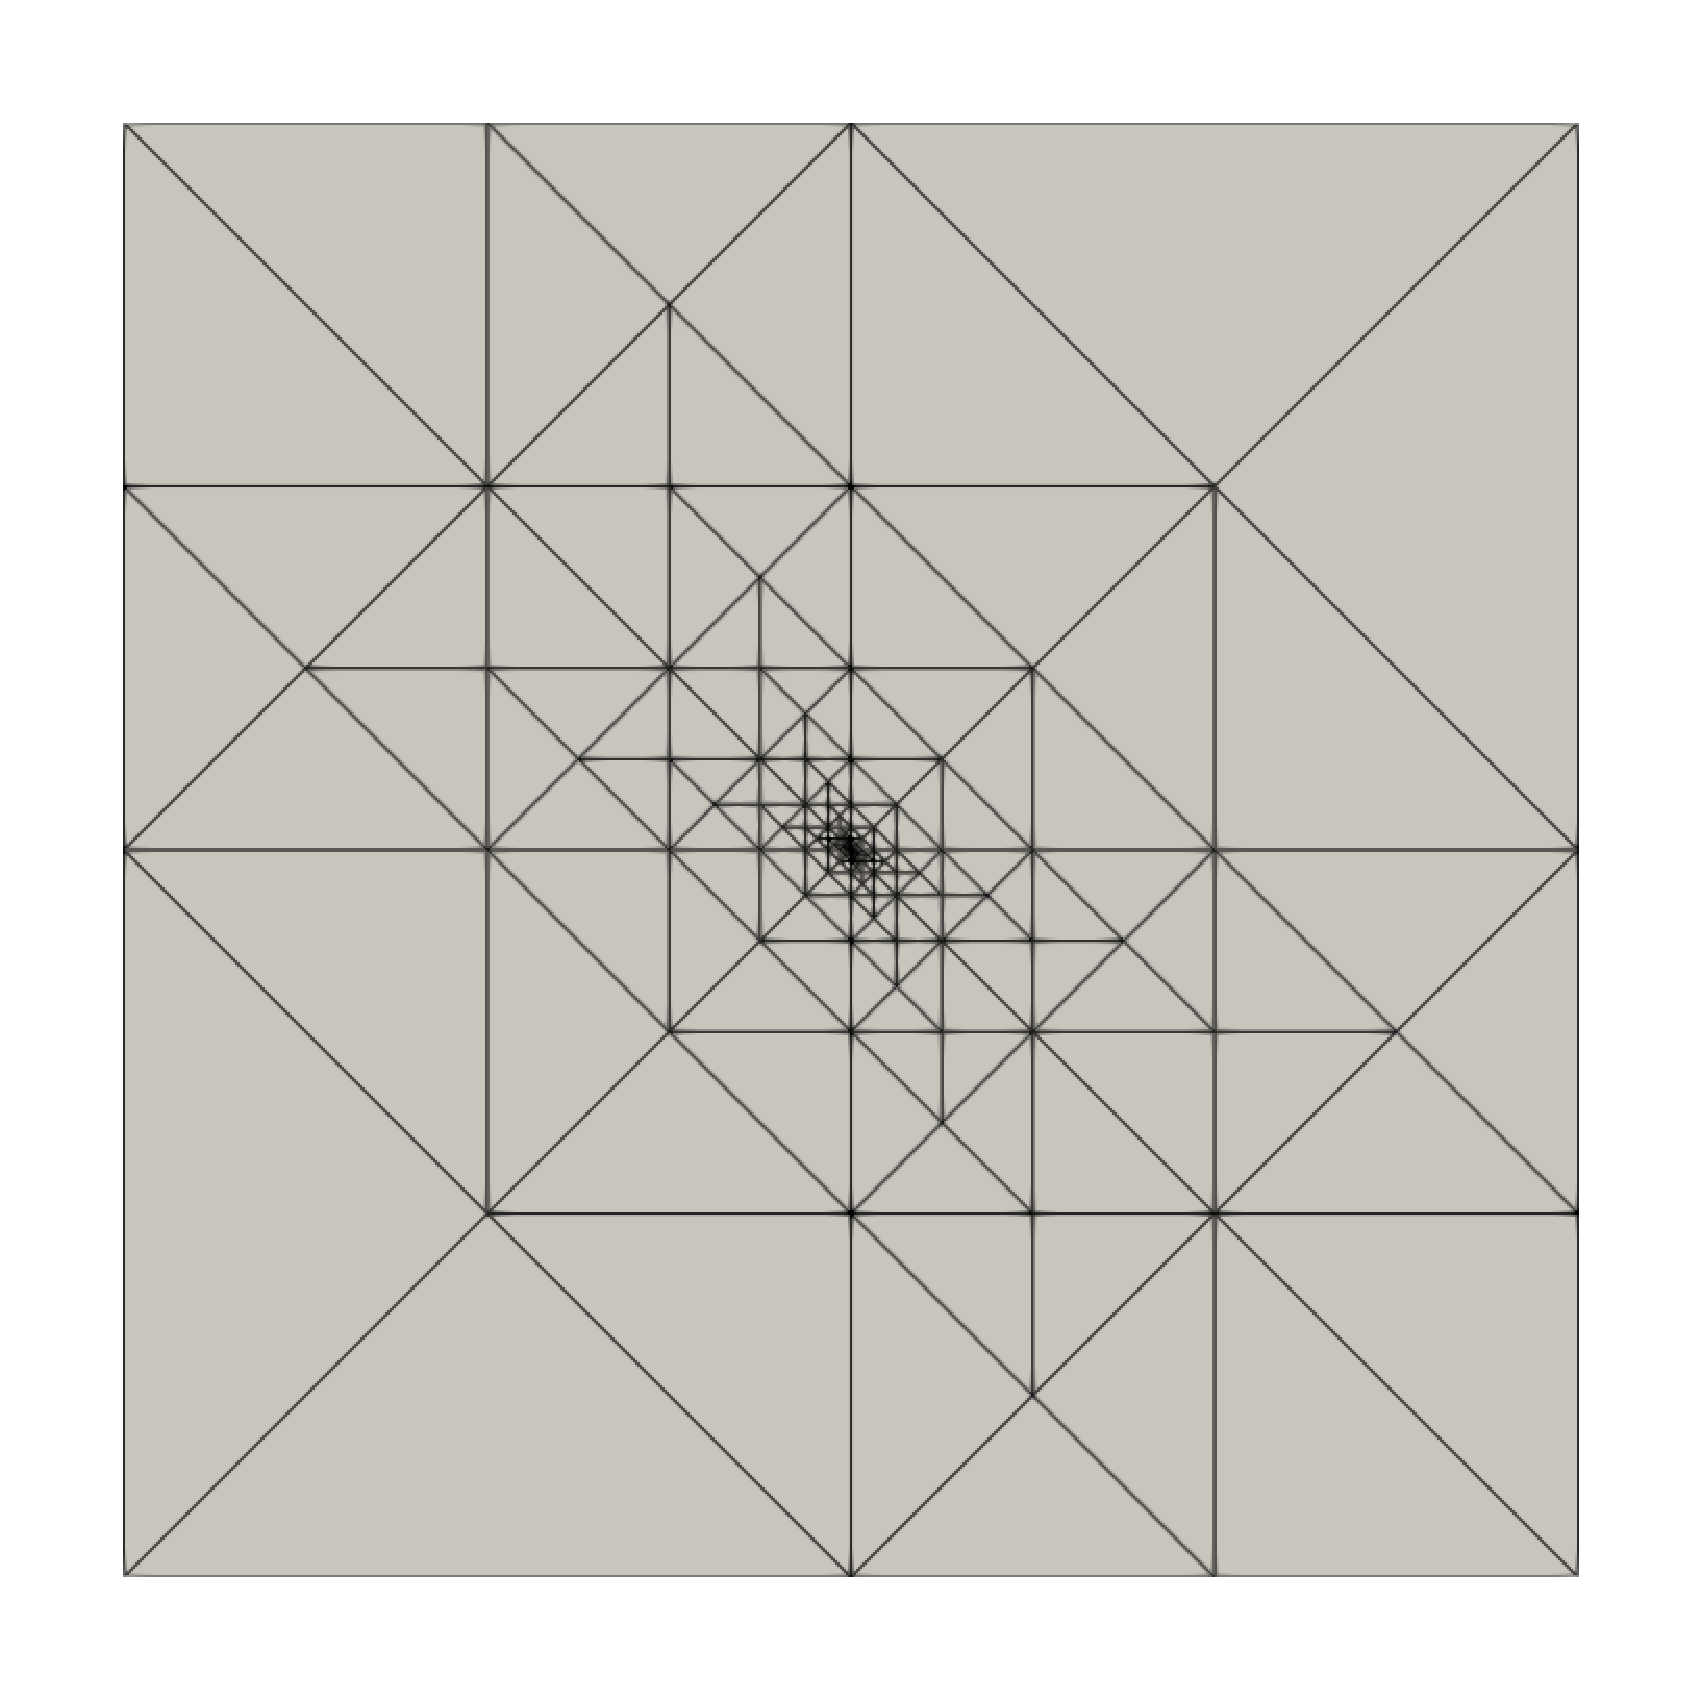
\includegraphics[width=\textwidth]{Riviere-100_P2_RT3_Mesh.pdf}
        \caption{}
        \label{fig:poisson-riviere_refmesh-p2}
    \end{subfigure}
    \caption{Results of adaptive FEM calculations with different orders $k$ and $m$. E.o.c and $\mathrm{i_{eff}}$ after the final refinement step are reported in (a).The two final meshes for $\kappa_1=100$ are depicted in (b) for $k=m-1=1$ and (c) for $k=m-1=2$.}
    \label{fig:poisson-riviere}
\end{figure}

\begin{wrapfigure}{r}{0.4\textwidth}
\centering
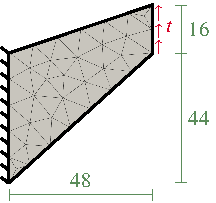
\includegraphics[scale=1.0]{fig_cooks-membrane.pdf}
\caption{Cooks membrane.}
\label{fig:cook_definition}
\end{wrapfigure}
\textbf{Example 2:} Based on the Poisson equation, the influence of the equilibration order $m$ on the efficiency of the resulting estimate is shown.
Using the Cooks membrane in Fig. \ref{fig:cook_definition}, this analysis is extended to linear elasticity, where the symmetry of the stress tensor is considered in a weak sense.
Within this analysis $\Pi_1=2.333$, $t=0.03$ and adaptive meshes based on a Dörfler marking strategy with $\theta=0.6$ are considered.
Characteristics of the first mesh fulfilling $\vert\vert\vert \Displacement - \Displacement_\h \vert\vert\vert \leq 10^{-3}$ are summarised in Fig. \ref{fig:cook_results-summary}. As $\LinPKEqlbH$ exactly fulfils the divergence condition from Definition \ref{def:equilibrated_stress}, $\eta$ reduced to the sum of the $\mathcal{A}$-norm of the stress difference $\LinPKEqlbH - \stressPKLin_\h$ and the norm of asymmetric part of $\LinPKEqlbH$. 
Following \ref{fig:cook_results-summary}, the estimate is clearly dominated by the second part.
Using equilibrated stresses of order $m=k+1$ increases the efficiency, with a relative reduction (compared to the case with $m=k$) comparable to those from the Poisson example.
An increased accuracy of the error estimate affects the effectivity of the adaptive solution procedure -- measured by the number of degrees of
freedom, required for a certain error -- in a positive way.
This trend is clearly much more pronounced for $k=2$, whereby a similar accuracy is achieved with $47\%$ fewer degrees of freedom.
A practical shortcut -- equilibration for $m=k+1$ is significantly more expensive than for $m=k$ -- seems to be the heuristic error indicator
\begin{eqnarray}
    \eta = \norm{\LinPKEqlbH - \stressPKLin_\h}\; ,
    \label{eq:elasticity_heuristic-ei}
\end{eqnarray}
where no weak symmetry is enforced on $\LinPKEqlbH$.
This yields efficiency indices close to one (see Fig. \ref{fig:cook_results-summary}), and shows, comparing the convergence history in Fig. \ref{fig:cook_results-convhist}, slightly better results as the guaranteed estimate with $m=k+1$.
\begin{figure}
    \centering
    \begin{subfigure}[b]{0.4\textwidth}
        \begin{tabular}{@{}l|c|c|ccc|l@{}}
            \toprule
            $k$ & $m$ & $n_\mathrm{DOF}$ & $\mathrm{err}$ & $\eta$ & $\eta _\mathrm{as}$ & $\mathrm{i_{eff}}$ \\ \midrule
            2 & 2 & 34070 & $0.0009$ & $0.009$ & $0.009$ & $10.7$ \\
            2 & 3 & 23202 & $0.0010$ & $0.008$ & $0.007$ & $7.9$ \\
            3 & 3 & 6656  & $0.0009$ & $0.020$ & $0.016$ & $17.0$ \\
            3 & 4 & 7100  & $0.0007$ & $0.009$ & $0.009$ & $13.0$ \\ \midrule
            2 & $2^*$ & 27788 & $0.0008$ & $0.001$ & $-$ & $1.5$ \\
            2 & $3^*$ & 26538 & $0.0008$ & $0.001$ & $-$ & $1.2$ \\
            3 & $3^*$ & 5738  & $0.0009$ & $0.001$ & $-$ & $1.5$ \\
            3 & $4^*$ & 5996  & $0.0008$ & $0.001$ & $-$ & $1.2$ \\ \bottomrule
        \end{tabular}
        \vspace{1.1cm}
        \caption{}
        \label{fig:cook_results-summary}
    \end{subfigure}
    \hfill
    \begin{subfigure}[b]{0.58\textwidth}
        \centering
        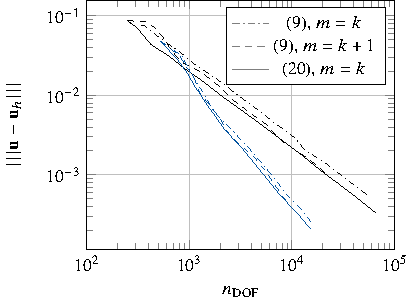
\includegraphics[scale=1.0]{fig_cook-convhistory.pdf}
        \caption{}
        \label{fig:cook_results-convhist}
    \end{subfigure}
    \caption{Effectivity of the different adaptive solution procedures for the Cooks membrane: (a) summarises the results for the first mesh with $\mathrm{err} = \vert\vert\vert \Displacement - \Displacement_\h \vert\vert\vert \leq 10^{-3}$, (b) details the convergence history (black: $k=2$, blue: $k=3$). Orders $m^*$ indicate the use of \eqref{eq:elasticity_heuristic-ei}}
    \label{fig:linelast-cook_results}
\end{figure}

Up to this point only the accuracy of the error estimates has been compared. 
Within the following the focus will be on the total solution time $t_\mathrm{tot}$, which is made up from $t_\mathrm{prime}$ -- the time for assembly and solution, using PETSc and MUMPS, of the primal problem -- and $t_\mathrm{eqlb}$, the time for performing the equilibration.
Comparing in a first step the relative equilibration costs $t_\mathrm{eqlb}/t_\mathrm{tot}$ for the Cooks membrane with fixed meshes in Fig. \ref{fig:cook_performance-uniform}, $t_\mathrm{eqlb}$ is -- for a sufficient size of the primal problem -- considerably smaller than $t_\mathrm{prime}$.  
Increasing $k$ increases the effort required for equilibration, while using an equilibration with $m=k+1$ is significantly more expensive than the respective lowest order case $m=k$. Similar timings for the adaptive solution of the Cooks membrane (timings are accumulated until $\vert\vert\vert \Displacement - \Displacement_\h \vert\vert\vert \leq 10^{-3}$) are summarised in Fig. \ref{fig:cook_performance-adaptive}.
While for the cases $k=m=2$ the total solution time is dominated by the solution of the primal problem, this trend is reversed for the more accurate (guaranteed) estimate with $k=m-1=2$.
Even though having the fewest primal degrees of freedom, the entire solution time is the highest due to the high computational costs for the equilibration.
Using primal approximations based on $k=3$ reduces the overall computation time, but leading to a significant share of the equilibration in the total computation time. 
An effect, amplified by the small sizes of the primal problems.
As for $k=2$ the heuristic indicator \eqref{eq:elasticity_heuristic-ei} with $m=k$ performs best, while the higher order estimate with $m=k+1$ is outperformed.
Clearly these results will have to be reevaluated in a parallel context -- which is beyond the current scope -- and also for primal problems of larger size.
\begin{figure}[]
\centering
    \begin{subfigure}[b]{0.6\textwidth}
        \centering
        \begin{tabular}{@{}c|ccc||c|ccc@{}}
        \toprule
        \multicolumn{4}{c}{$k=2$}    & \multicolumn{4}{c}{$k=3$}    \\ \midrule
        $n_\mathrm{DOF}\,\setminus\, m$ & 2    & $2^*$    & 3    & $n_\mathrm{DOF} \,\setminus\, m$ & 3    & $3^*$    & 4    \\ \midrule
        $3.49 \cdot 10^3$  & 36.3 & 27.4 & 66.4 & $3.31 \cdot 10^3$ & 45.4 & 37.9 & 63.1 \\
        $1.36 \cdot 10^4$  & 22.0 & 15.1 & 49.4 & $1.30 \cdot 10^4$ & 33.6 & 27.0 & 51.7 \\
        $2.14 \cdot 10^5$  & 15.3 & 10.2 & 38.6 & $2.04 \cdot 10^5$ & 24.5 & 19.3 & 40.9 \\
        $8.54 \cdot 10^5$  & 12.6 & 8.34 & 33.7 & $8.13 \cdot 10^5$ & 20.7 & 16.2 & 35.6 \\ \bottomrule
        \end{tabular}
        \vspace{0.2cm}
        \caption{}
        \label{fig:cook_performance-uniform}
    \end{subfigure}
    \hfill
    \begin{subfigure}[b]{0.38\textwidth}
        \centering
        \begin{tabular}{@{}l|c|ccc@{}}
            \toprule
            $k$ & $m$ & $t_\mathrm{prime}$ [s] & $t_\mathrm{tot}$ [s] & ratio [\%] \\ \midrule
            2 & 2     & $0.47$ & $0.61$ & 23.2\\
            2 & $2^*$ & $0.38$ & $0.45$ & 16.4\\
            2 & 3     & $0.31$ & $0.65$ & 52.7 \\ \midrule
            3 & 3     & $0.09$ & $0.15$ & 41.9\\
            3 & $3^*$ & $0.07$ & $0.11$ & 35.6\\
            3 & 4     & $0.10$ & $0.26$ & 60.5\\ \bottomrule
        \end{tabular}
        \caption{}
        \label{fig:cook_performance-adaptive}
    \end{subfigure}
    \caption{Performance measurements based on the Cooks membrane. (a) $\mathrm{ratio} = t_\mathrm{eqlb} / t_\mathrm{tot}$ in $\%$ for different primal problems. (b) Accumulated timings using an adaptive algorithm until $\vert\vert\vert \Displacement - \Displacement_\h \vert\vert\vert \leq 10^{-3}$. Orders $m^*$ indicate the use of \eqref{eq:elasticity_heuristic-ei}.}
    \label{fig:linelast-cook_performance}
\end{figure}

\section*{Conclusions}
Within this contribution dolfinx\_eqlb, a FEniCSx based library for the efficient equilibration of fluxes and stresses, has been introduced. 
Characteristic examples for the Poisson problem and linear elasticity highlight the applicability of the library.
Additionally, an efficient, but heuristic error indicator for elasticity is introduced, neglecting the asymmetry of the equilibrated stress.
Within our future work the efficiency of the presented implementation as well as the heuristic error indicator for real world problems has to be proven. 
We further intend to generalise the implementation to 3D domains and multi-physical problems like poroelasticity.
\vspace{-0.1cm}
\subsection*{Supplementary material}
This work is based on dolfinx\_eqlb v1.2.0 (\url{https://github.com/brodbeck-m/dolfinx_eqlb/tree/v1.2.0}). 
The presented examples can either be accessed via GitHub (\url{https://github.com/brodbeck-m/AFEM-by-Equilibration}) or, containing a Docker image, \cite{DatsetPaper}.
\vspace{-0.1cm}
\bibliographystyle{spbasic}
\bibliography{chapters/brodbeck/bibliography.bib}


